%=============================================================================80
% Template taken and edited from:
% https://www.overleaf.com/latex/templates/emory-poster-template/skpfmpxjnqdh
% When compiling, you need "emory-theme.sty" and "refs.bib" to be in the same
% directory as "main.tex".
% I chose not to include "refs.bib" but using it is recommended.
%
% Compile in the following order from top to bottom:
% $ pdflatex main.tex
% $ biber main.bcf
% $ pdflatex main.tex
% $ pdflatex main.tex
%=============================================================================80
\documentclass[20pt,margin=1in,innermargin=-4.5in,blockverticalspace=-0.25in]{tikzposter}
\geometry{paperwidth=42in,paperheight=30in}
\usepackage[utf8]{inputenc}
\usepackage{amsmath}
\usepackage{amsfonts}
\usepackage{amsthm}
\usepackage{amssymb}
\usepackage{mathrsfs}
\usepackage{graphicx}
\usepackage{subfigure}
\usepackage{float}
\usepackage{enumitem}
\usepackage{braket}
\usepackage[backend=biber,style=numeric]{biblatex}
\usepackage{emory-theme}

\usepackage{mwe} % for placeholder images
\newcommand{\bem}{\begin{pmatrix}}
\newcommand{\enm}{\end{pmatrix}}

% set theme parameters
\tikzposterlatexaffectionproofoff
\usetheme{EmoryTheme}
\usecolorstyle{EmoryStyle}

\title{Visualization of Electronic Transitions Using Natural Transition Orbitals}
\author{Alan Robledo}
\institute{Department of Physics and Astronomy, University of California, Irvine}
\titlegraphic{
\includegraphics[width=0.06\textwidth]{uci-seal.png}}

% begin document
\begin{document}
\maketitle
\centering
\begin{columns}
    \column{0.3}
    \block{Introduction}{
         The objective is to describe electronic excitations in diatomic molecules modeled by a morse potential and a harmonic potential (see figure below) using the electron-hole picture.
         By considering the Configuration Interaction Singles approximation, natural transition orbitals (NTOs) can be constructed, as described by Plasser and Wormit [1], and used for visualizing an electronic transition.
         This consists of performing a Singular Value Decomposition (SVD) of the Transition Density Matrix (TDM) which requires obtaining forms of the wavefunctions associated with the transition.
         NTOs are especially useful in quantum chemistry because chemists are often interested in orbital representations of electron dynamics during chemical processes.
         \begin{tikzfigure}
             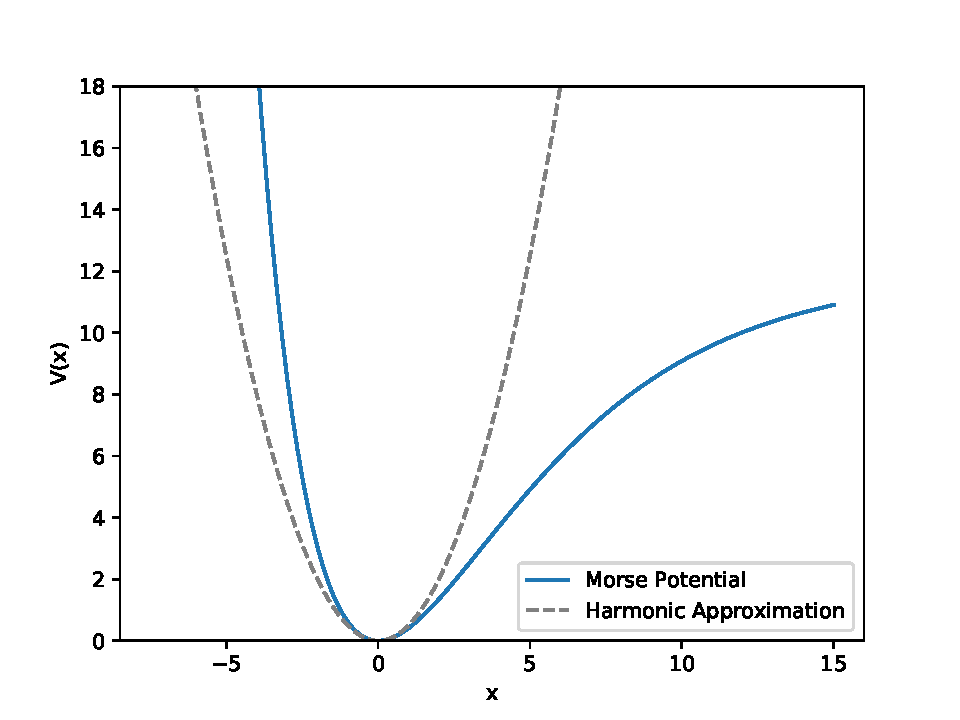
\includegraphics[width=1.0\linewidth]{../plots/morse_potential.pdf}
         \end{tikzfigure}
    }
    \block{Methods}{
      \begin{enumerate}
        \item \textbf{Schr\"odinger Equation}\\
        Performing an eigenvalue decompositon of the hamiltonian matrix $\hat{H}$ yields quantized energies $E_n$ and associated wavefunctions $\psi_n$.
        \begin{equation}
          \begin{split}
            \hat{H} \psi_n &= E_n \psi_n \\
            (\hat{T} + \hat{V}) \psi_n &= E_n \psi_n \\
            \Big[ - \frac{\hbar^2}{2m} \frac{\partial^2}{\partial x^2} + D_e (e^{- \omega_x x} - 1)^2 \Big] \psi_n &= E_n \psi_n
          \end{split}
        \end{equation}
        \item \textbf{Kinetic Energy}\\
        Discretize the partial derivative by creating a uniform grid with spacing $\Delta = x_{i+1} - x_{i}$. Using the central-difference formula,
        \begin{equation}
          f'(x) = \frac{\partial}{\partial x} f(x) \approx \frac{f(x_{i+1}) - f(x_{i-1})}{2 \Delta}
        \end{equation}
        a form for the second derivative can be derived
        \begin{equation}
          f''(x) = \frac{\partial^2}{\partial x^2} f(x) \approx \frac{f(x_{i+1}) - 2 f(x_i) + f(x_{i-1})}{\Delta^2} .
        \end{equation}\\
      \end{enumerate}
    }

    \column{0.34}
    \block{}{
      This gives a system of linear equations which allows us to write the kinetic energy in matrix form as
      \begin{equation}
        - \frac{\hbar^2}{2m} \frac{\partial^2}{\partial x^2} f(x) \approx - \frac{\hbar^2}{2m} \frac{1}{\Delta^2} \bem -2 & 1 & 0 & 0 & 0 & \cdots \\ 1 & -2 & 1 & 0 & 0 & \cdots \\ 0 & 1 & -2 & 1 & 0 & \cdots \\ 0 & 0 & 1 & -2 & 1 & \cdots \\ & & \vdots & & & \enm \bem \vdots \\ f(x_{i-1}) \\ f(x_i) \\ f(x_{i+1}) \\ \vdots \enm
      \end{equation}
      \begin{enumerate}
        \setcounter{enumi}{2}
      \item \textbf{Potential Energy}\\
      If we think of our real-space grid as delta functions sitting on lattice points in 1D, i.e., $\ket{x_i} = \delta(x - x_i)$, the potential energy matrix becomes a diagonal matrix where the i-th element along the diagonal is $V(x_i)$.
      \item \textbf{NTOs}\\
      We want a compact way to store the information regarding electronic excitations in our system. We can do this by performing a singular value decomposition
    of the transition density matrix $\Gamma$. An element of the TDM can be computed as
    \begin{equation}
      \Gamma_{nm} = \braket{n|\Gamma(x, x')|m} = \int dy dy' \delta(x - y) \phi_n^*(y) \phi_m(y') \delta(x' - y')
    \end{equation}
    Performing an SVD of the TDM gives
    \begin{equation}
      \Gamma = \textbf{U} \Sigma \textbf{V}^{\textbf{T}}
    \end{equation}
    where \textbf{U} is a matrix of coefficients that describe the hole and \textbf{V} is a matrix of coefficients that describe the particle. $\Sigma$ is a pseudo-diagonal matrix of singular values that describe the amount of contribution an NTO pair has on any given transition.
    \end{enumerate}
    }

    \block{Results}{
        \vspace{-2cm}
        \begin{tikzfigure}
            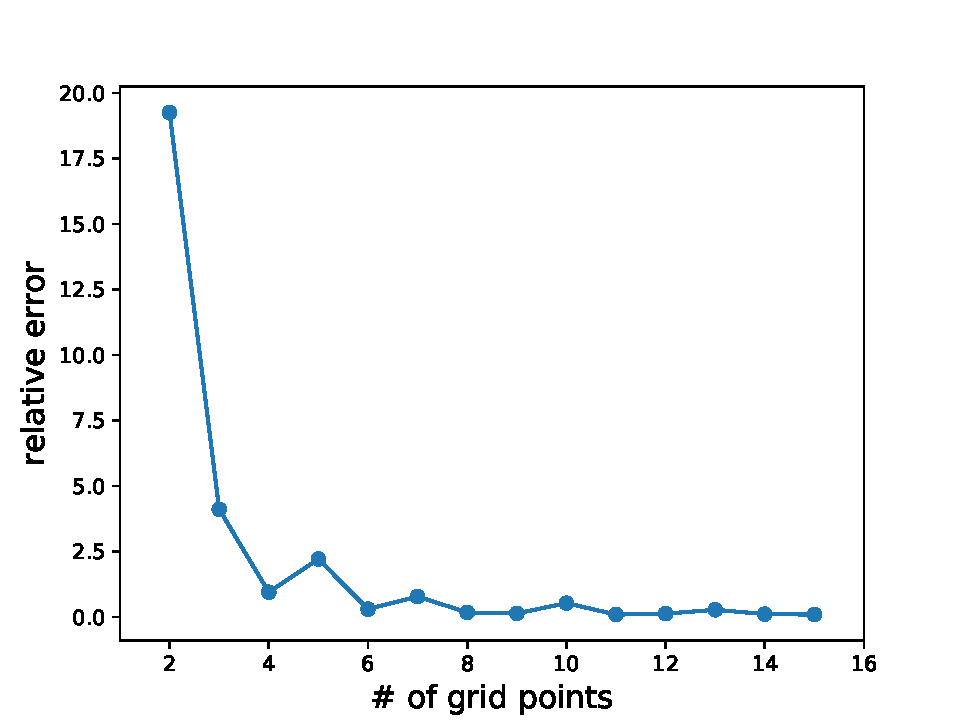
\includegraphics[width=0.8\linewidth]{../plots/energy_error.pdf}
        \end{tikzfigure}
        \begin{itemize}
          \item Values of $\hbar = 1$, $m = 1$, $\omega_x = 0.2041241$ and $D_e = 12$ were used to compare computed energies with those obtained from calculations by Garashchuk [2]. Ground state energy calculations were also compared to the analytic solution: \\
          \begin{equation}
            E_n = h \nu \Big(n + \frac{1}{2} \Big) - \frac{[h \nu( n +\frac{1}{2})]^2}{4 D_e} .
          \end{equation}
          \item Increasing the number of grid points gives more accurate results but also increases CPU time. Computing energies with 50 grid points takes 0.843 seconds. Computing energies with 500 grid points takes 0.990 seconds. Computing energies with 5000 grid points takes 2 minutes and 35.431 seconds.
        \end{itemize}
        \vspace{-1cm}
    }

    \column{0.34}
    \block{}{
    \vspace{-3cm}
    \begin{figure}[H]
      \hspace{-4cm}
      \begin{subfigure}
          \centering
          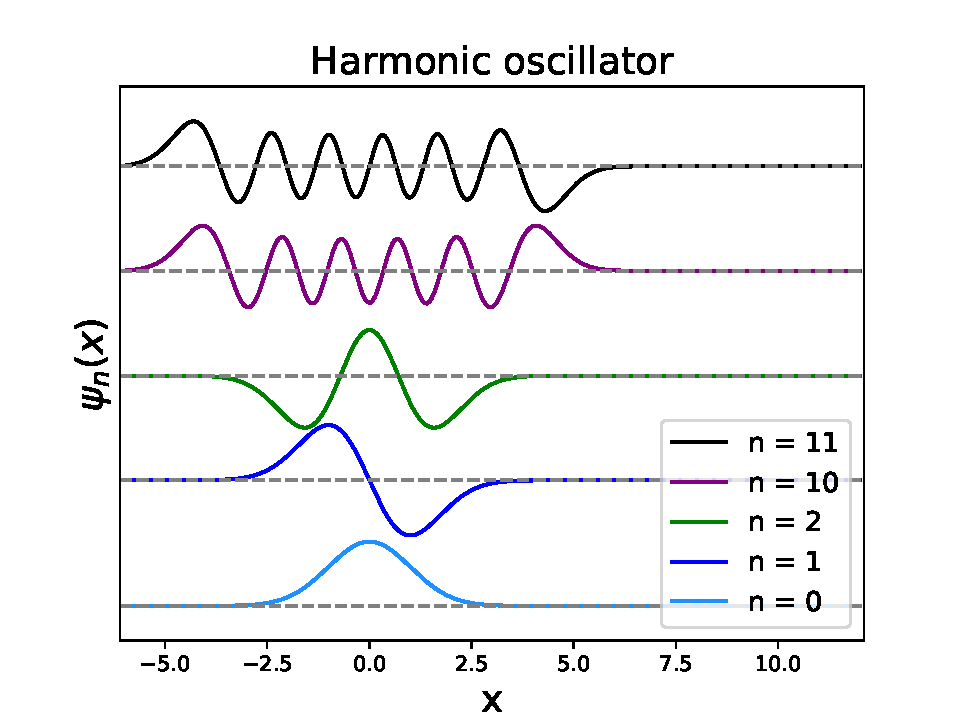
\includegraphics[height=6.0in]{../plots/harmonic_states.pdf}
      \end{subfigure}
      \hspace{-2.0cm}
      \begin{subfigure}
          \centering
          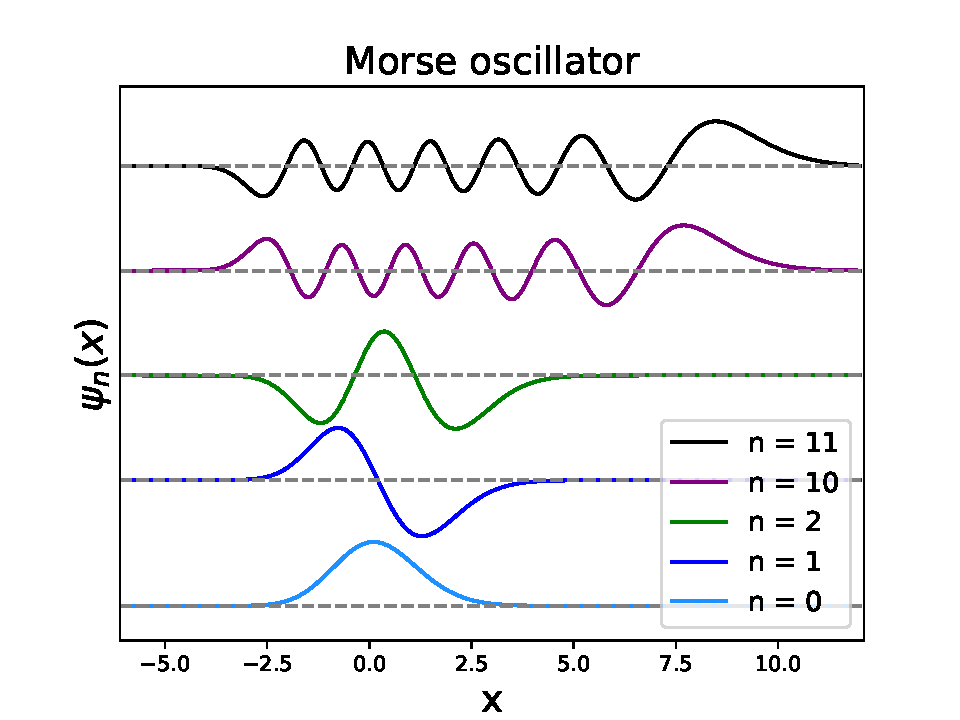
\includegraphics[height=6.0in]{../plots/morse_states.pdf}
      \end{subfigure}
    \end{figure}
    \vspace{-1cm}
    \begin{itemize}
      \item Wavefunctions for the morse potential should look similar to those of the harmonic potential because the harmonic potential is a good approximation to the morse potential for small displacements around the equilibrium position.
      \item Issues occured with the numpy/scipy eigenvalue solver. Running the same script on different versions of Python yielded eigenvectors that were different by a minus sign. This created inconsistencies with plotting the wavefunctions but minus signs cancelled out when plotting probability densities.
    \end{itemize}
    \vspace{-1cm}
    \begin{figure}[H]
      \hspace{-4.0cm}
      \begin{subfigure}
          \centering
          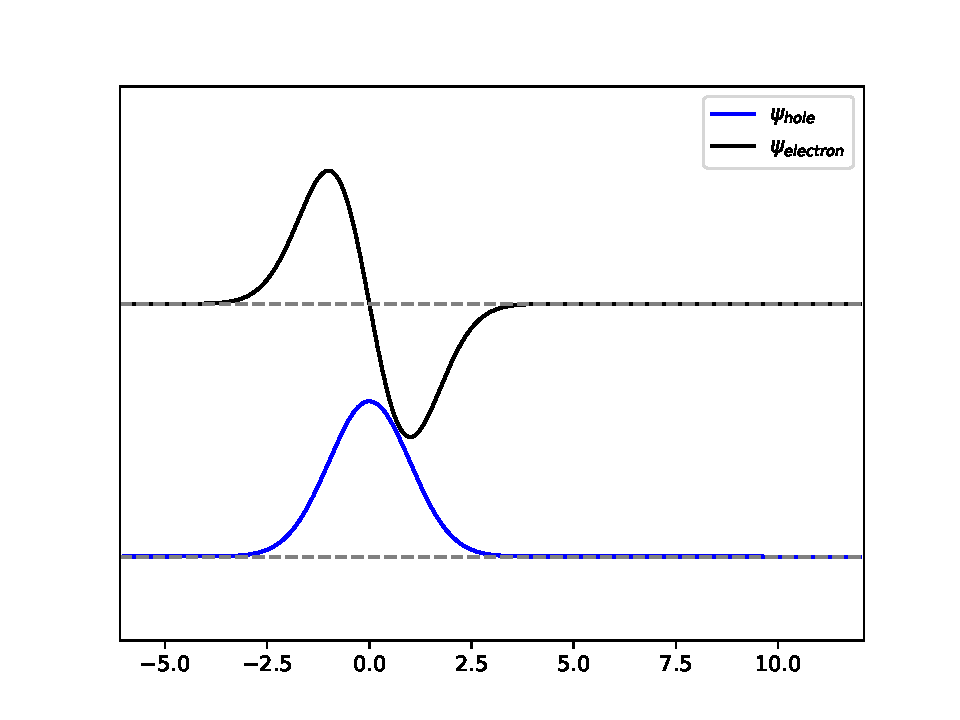
\includegraphics[height=6.0in]{../plots/harmonic_ntos.pdf}
      \end{subfigure}
      \hspace{-2.5cm}
      \begin{subfigure}
          \centering
          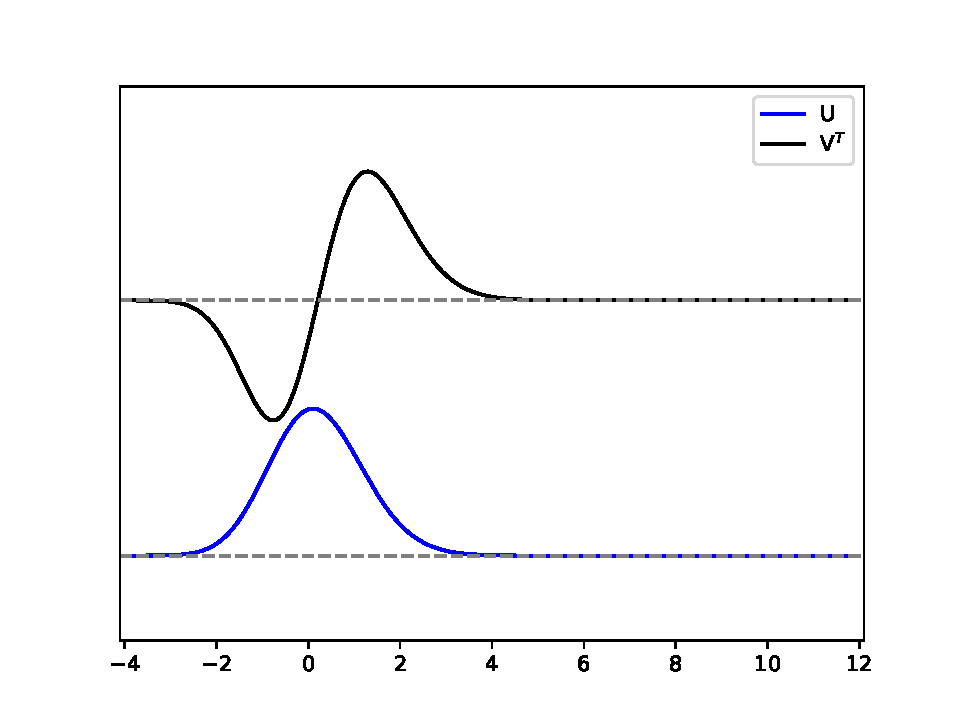
\includegraphics[height=6.0in]{../plots/morse_ntos.pdf}
      \end{subfigure}
    \end{figure}
    \begin{itemize}
      \item For the harmonic potential case, a transition density matrix was created between the ground state and the second excited state. After performing an SVD, the first column of the \textbf{U} matrix contained the hole NTO and the first row of the \textbf{V}$^{\text{\textbf{T}}}$ matrix contained the electron NTO because the first singular value was $\approx$ 1. This means that contributions from every other NTO pair to the excitation are virtually nonexistent.
      \item For the morse potential case, a transition density matrix was created between the ground state and the eleventh excited state. Like the harmonic case, the hole and electron NTOs were contained in the first column of the \textbf{U} matrix and the first row in the \textbf{V}$^{\text{\textbf{T}}}$ matrix respectively. This shows that the SVD method works very well in the configuration interaction singles case.
    \end{itemize}
    }

    \block{References}{
        [1] Plasser, F.; Wormit, M.; Dreuw, A. New tools for the systematic analysis and visualization of electronic excitations. I. Formalism. \textit{J. Chem. Phys.} \textbf{2014}, \textit{141}, 024106-(1-13).

        [2] Garashchuk, S.; Light, J. C. Quasirandom distributed Gaussian bases for bound problems. \textit{J. Chem. Phys.} \textbf{2001}, \textit{114}, 3929-3939.
    }

\end{columns}
\end{document}
